\section{Ausstattung Labor}
\label{sec:Ausstattung_Labor}

Das Praktikum wird im Labor für Echtzeitsysteme (EZS Labor) der Hochschule Niederrhein durchgeführt.

\begin{center}
	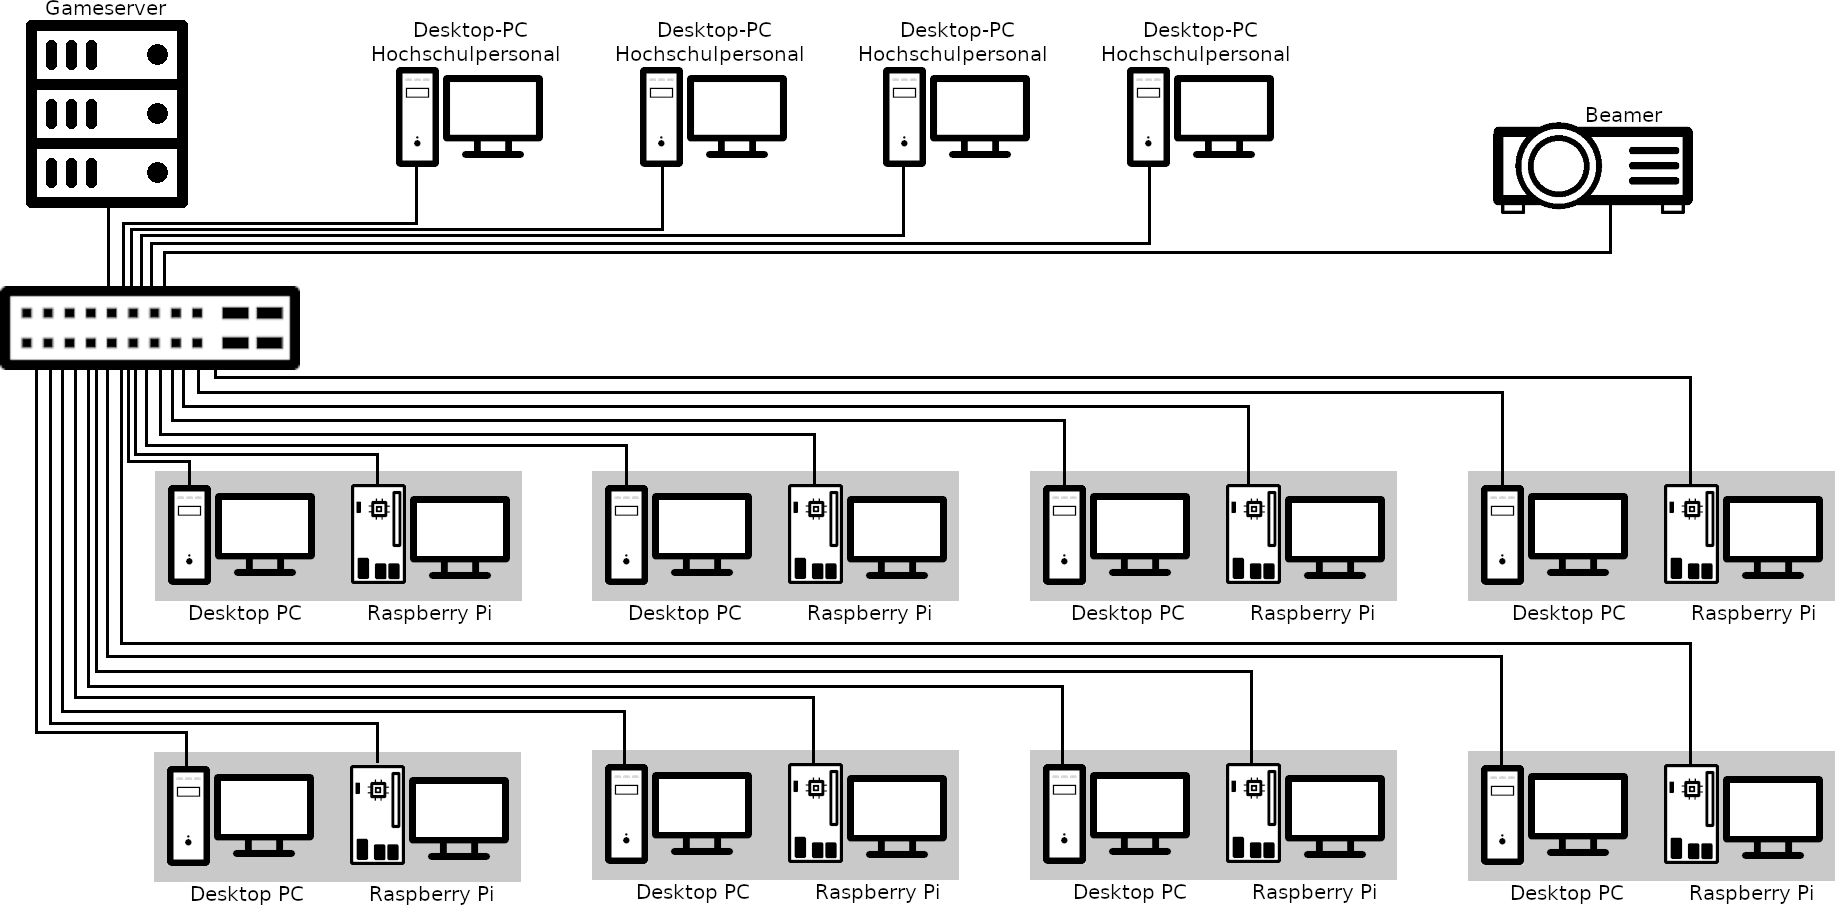
\includegraphics[width=\linewidth, keepaspectratio]{analyse/netzwerk-topologie-bak}
	\captionof{figure}{Übersicht über die Laborausstattung (Netzwerktopologie)}
	\label{fig:network-topology}
\end{center}

Wie in der Abbildung \ref{fig:network-topology} zu sehen, ist das Labor mit acht Gruppenarbeitsplätzen für Studierende sowie Arbeitsplätzen für die Betreuer und Mitarbeiter ausgestattet. Ein Betreuerarbeitsplatz kann zu einem neunten Gruppenarbeitsplatz umfunktioniert werden.

An einem Gruppenarbeitsplatz (in der Abbildung \ref{fig:network-topology} grau hinterlegt) können 2 Studierende gleichzeitig arbeiten, da diese mit einem leistungsfähigen Desktop-PC und einem Raspberry Pi\footnote{Einplatinencomputer mit der Größe einer Kreditkarte} sowie den dazugehörigen Peripheriegeräten (Maus, Tastatur \& Monitor) ausgestattet sind.

Als Betriebssystem wird auf den Desktop-PCs Ubuntu\footnote{Ubuntu ist eine freie Linux Distribution auf Basis von Debian} und auf den Raspberry Pis Raspbian\footnote{Abwandlung von Debian für den Raspberry Pi} verwendet.

Auf den Desktop-PCs ist die Software VirtualBox der Firma Oracle installiert. Diese ermöglicht das Virtualisieren eines weiteren Rechners. Diese Virtuelle Maschine wird Gast genannt und beheimatet die Dienste und Anwendungen, welche während des Versuchs benötigt werden. Durch die Nutzung der Virtualisierung muss die Software nicht auf dem Wirtsystem installiert werden. So ist dieses auch für andere Versuche im Rahmen der Lehrveranstaltung nutzbar, ohne das auf Inkompatibilitäten von Softwares der verschieden Versuche geachtet werden muss. Auch bietet VirtualBox die Möglichkeit sogenannte Snapshots anzulegen. Ein Snapshot ist eine Momentaufnahme eines aktuellen Systemzustandes. Diese stellt eine Komplettsicherung des Systems dar. Durch diese ist es möglich, die Systeme auf den gleichen Stand zu bringen. Dieses wird benötigt, um eine Vergleichbarkeit zwischen den Studierenden zu gewährleisten.\cite{oraclecorporationOracleVMVirtualBox2020}

Die teilnehmenden Studentengruppen werden in den Softwarekomponenten und in der Auswertung durch die IP-Adresse ihres Gast-Systems identifiziert.

Neben diesen Rechner steht ein Linux Server zur Verfügung, auf welchem das Auswertungs- und Überwachungssystem betrieben wird.

Alle Rechner, auch die Gastsysteme der Studentengruppen, sind untereinander über ein Netzwerkswitch via Ethernet verbunden.

Außerdem steht ein Beamer zur Verfügung auf dem die aktuelle Spielübersicht dargestellt werden kann.